
% They just report mass flows
% or are proprietary and super long running

\begin{frame}[ctb!]
  \frametitle{Top Level Fuel Cycle Simulators}
  % most only report mass flows.
  \begin{figure}[htbp!]
    \begin{center}
      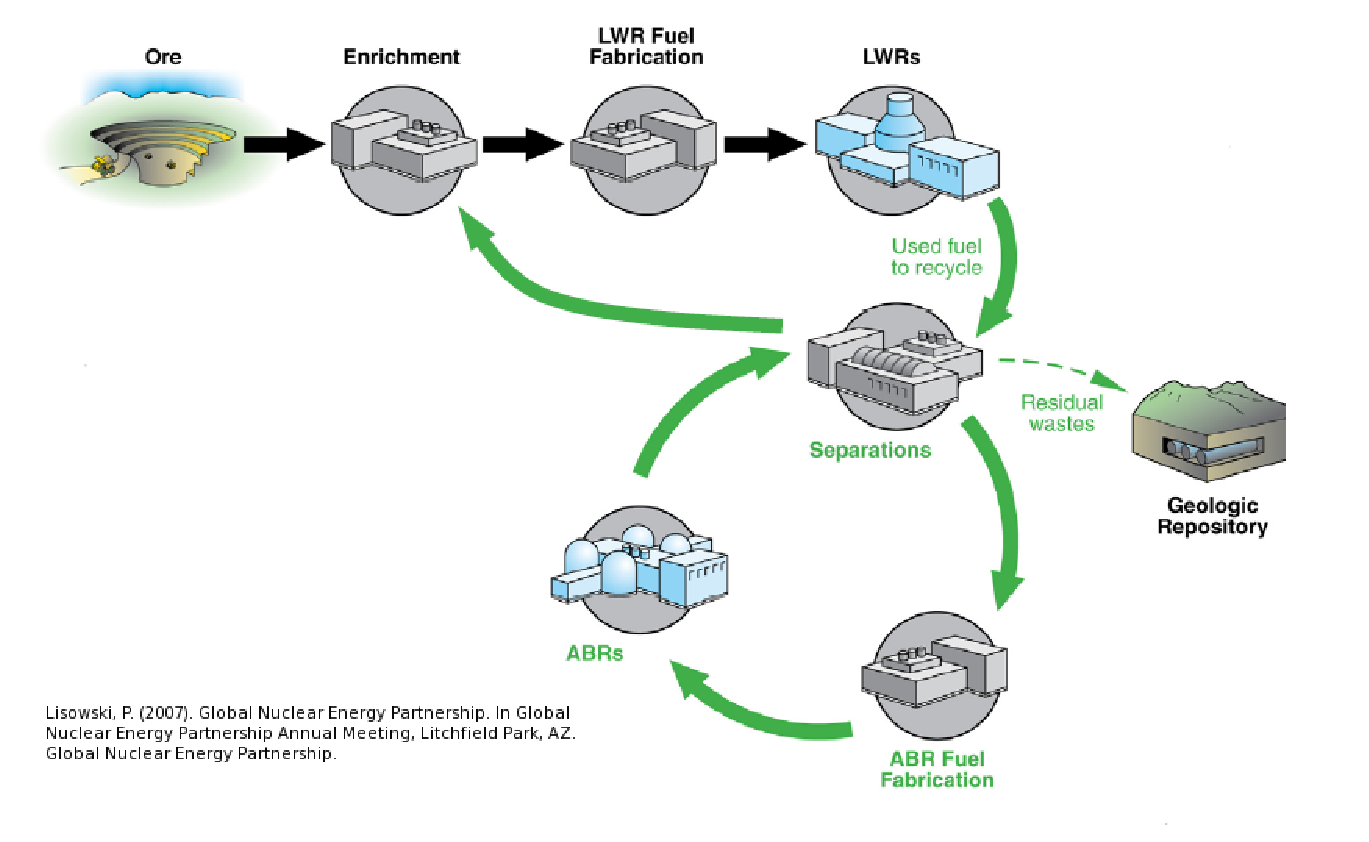
\includegraphics[height=4cm]{./images/simulations.eps}
    \end{center}
    \caption{Top level simulators are intended to model the collective 
    behavior of various fuel cycle decisions and 
    strategies \cite{lisowski_global_2007}.}
    \label{fig:simulation}
  \end{figure}
\end{frame}

\begin{frame}[ctb!]
  \frametitle{Need For an Integrated Repository Model}

  %        File: systools_tab.tex
%     Created: Mon Aug 29 09:00 AM 2011 C
% Last Change: Mon Aug 29 09:00 AM 2011 C
%
\begin{table}
  \centering
  \footnotesize{
  \begin{tabular}{|l|l|c|c|c|}
    \multicolumn{5}{c}{\textbf{Repository Capabilities within Systems Analysis Tools}}\\
    \hline
    Tool & Institution & Fuel Disposition & Radionuclide Transport & Heat Transport  \\
    \hline
    NUWASTE\cite{abkowitz_nuclear_2010} & NWTRB & yes & no & no \\
    VISION \cite{yacout_vision_2006} & INL   & yes & no & YMR only \\
    DANESS \cite{van_den_durpel_daness:_2006} & ANL   & no & no & no \\
    COSI   \cite{boucher_international_2010} & CEA   & yes & no & yes \\
    NFCSim \cite{schneider_nfcsim_2004} & LANL  & no & no & no \\
    CAFCA  \cite{guerin_benchmark_2009} & MIT   & no & no & no \\
    ORION  \cite{guerin_benchmark_2009} & BNL   & no & no & no \\
    TSM    \cite{turner_discrete_2010} & OCRWM & yes & no & YMR only \\
    \hline
  \end{tabular}
  \caption[System Tools]{System tools are lacking in radionuclide transport and  
  heat transport calculations in generic geolgies.}
  \label{tab:systools}
  }
\end{table}



An integrated repository performance model enables the analysis of global fuel 
cycle metrics concerned with material routing, intermediate storage time, and 
repository performance. Post-processed analysis of these metrics can neglect 
feedback effects of geologic disposal capacity constraints and repository 
performance within the fuel cycle system.

\end{frame}

